Utilizzare sistemi IDS e IPS in una rete risulta vantaggioso per diverse ragioni. Gli IDS/IPS hanno un buon grado di conoscenza dei livelli applicativi, (a differenza del firewall la cui competenza si ferma ai livelli 3 e 4 della pila ISO-OSI) possono investigare i pacchetti e sono istruiti in modo da riconoscere eventuali pattern di attacco noti sfruttando delle strategie di detection signature-based, behaviour-based e policy-based.
Viene ora posta l'attenzione su un particolare NIDS/NIPS chiamato Snort, un software nato nel 1998 diventato molto popolare e diffuso grazie alla sua usabilità e al fatto di essere open source. Sfrutta una strategia di detection rule-based (basato su regole), leggermente differente rispetto alle tecniche descritte in precedenza. A differenza delle firme, le regole si basano sull'identificazione della vulnerabilità effettiva, non di un exploit. Questo tipo di rilevamento è in genere classificato come ``0-day detection'', perché non è necessario che il virus abbia infettato qualcuno per scrivere una regola, bensì è sufficiente una comprensione approfondita delle vulnerabilità. Snort ha una community vasta e questo permette di aggiornare continuamente le rules. Non appena viene scritta una nuova regola tutta la community ne potrà beneficiare semplicemente facendo un aggiornamento ~\cite{snort}.

\section{Definizione}

Snort è un software open source rule-based che permette di rilevare e prevenire intrusioni in una LAN. A seconda di come configurato può generare alert che avvisano gli utenti, oppure può intraprendere azioni attive sui pacchetti sospetti bloccandone il transito. Le regole possono essere scritte/modificate da un amministratore oppure possono essere utilizzate direttamente le rules offerte dalla community. In entrambi i casi è possibile adattarle alle esigenze e ai servizi della propria rete. Inoltre Snort è in grado di combinare più strategie di detection. Oltre alla gestione delle rules può eseguire analisi di protocollo (policy-based detection) o studiare le anomalie (behaviour-based detection). Un esempio può essere l'analisi del protocollo TCP. Se dei pacchetti di SYN contenessero dei dati, o venissero ricevuti dei dati al di fuori della finestra di ricezione, allora verrebbe segnalata un'attività sospetta all'amministratore.

\begin{figure}[h]
    \begin{center}
        \begin{tabular}{l}
            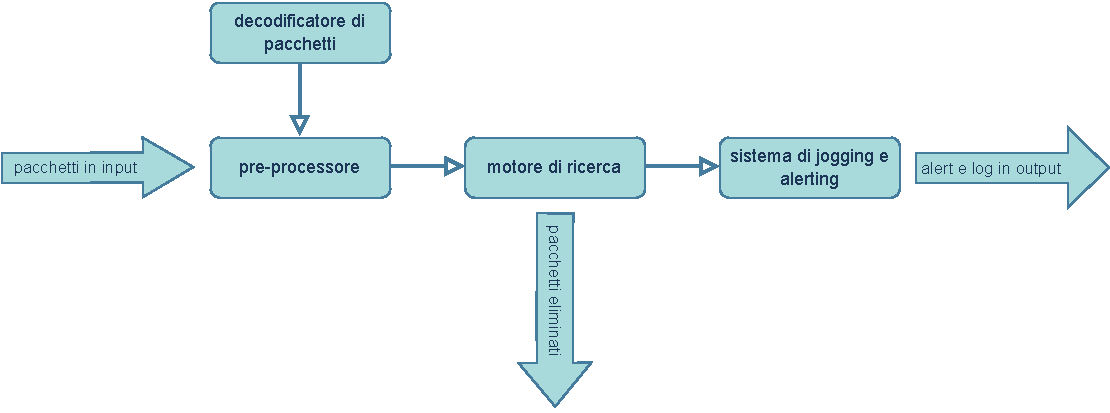
\includegraphics[width=14cm]{figure/components_of_snort.pdf}
        \end{tabular}
    \end{center}
    \caption{Componenti di Snort}
\end{figure}

I componenti principali di Snort sono citati brevemente:
\begin{itemize}
    \item \textbf{Decodificatore di pacchetti}  preleva i pacchetti da varie interfacce di rete e li prepara per la pre-elaborazione.
    \item \textbf{Pre-processori}  identifica gli header dei protocolli al livello di datalink, di rete, di trasporto e di applicazione. Si occupa del riassemblaggio dei pacchetti e del flusso TCP.
    \item \textbf{Motore di ricerca} componente principale che elabora e analizza i pacchetti applicando le regole. Confronta ogni pacchetto con un set di regole per vedere se esiste una corrispondenza.
    \item \textbf{Logging e alerting} sistema che si occupa della generazione di log e alert.
\end{itemize}

\section{Modalità di base}

Il comportamento di Snort nei confronti dei pacchetti varia a seconda della sua configurazione. Esistono diverse modalità di esecuzione che vengono presentate a seguire.

\subsection{Sniffer Mode}

Snort in sniffer mode ha un funzionamento analogo a tcpdump: sniffa il traffico che transita su un'interfaccia e lo stampa su console. Offre il riepilogo del traffico di rete alla fine dell'acquisizione. In questo modo vengono stampati con diversi livelli di dettaglio i contenuti dei pacchetti della suite TCP/IP, è possibile decidere di mostrare l'header, il payload o tutto il pacchetto. È importante sottolineare che per ora non sono state ancora introdotte regole, quindi Snort analizzerà e stamperà a schermo indiscriminatamente tutto il traffico presente sull'interfaccia.

I parametri che possono essere utilizzati sono:

\begin{itemize}
    \item \textbf{-i} per specificare l'interfaccia da sniffare.
    \item \textbf{-v} verbose.
    \item \textbf{-d} mostra il payload del pacchetto.
    \item \textbf{-e} mostra l'header del pacchetto.
    \item \textbf{-X} per fare il display di tutto il contenuto del pacchetto.
\end{itemize}

Un esempio di utilizzo è il seguente:

\begin{verbatim}
    snort -i ens160 -v.
\end{verbatim}

In questo modo partirà un'istanza di Snort che analizzerà il traffico sull'interfaccia ens160 e lo stamperà su console in verbose mode.

\subsection{Packet Logger Mode}

Il passaggio successivo allo sniffing dei pacchetti è la loro registrazione. Snort eseguito in packet logger mode memorizza su disco il traffico rilevato. La directory predefinita di Snort è \texttt{/var/log/snort}. Se i log venissero memorizzati solo in formato ASCII la directory di registrazione potrebbe diventare molto congestionata nel tempo, a causa del numero sempre crescente di directory e file. Registrare il traffico di una rete molto attiva potrebbe portare ad esaurire gli inode (una struttura dati Unix che limita il numero totale di file in un file system) molto prima di esaurire lo spazio di archiviazione. Questa esplosione di file può mettere a dura prova la macchina e potrebbe finire per trasformarsi in un vero e proprio attacco DoS. Per questo i log vengono registrati in binario e poi all'occorrenza vengono convertiti in formato ASCII per essere letti dall'amministratore.

I parametri che possono essere utilizzati sono:

\begin{itemize}
    \item \textbf{-l} permette di specificare la directory dove si vogliono memorizzare i log.
    \item \textbf{-k ASCII} i log vengono memorizzati nel formato più leggibile per l'utente. Quando Snort viene eseguito in questa modalità, raccoglie ogni pacchetto che vede e lo colloca in una gerarchia di directory basata sull'indirizzo IP degli host.
    \item \textbf{-r} opzione per leggere i log memorizzati in binario.
    \item \textbf{-n} specifica il numero dei pacchetti da leggere.
\end{itemize}

I vari parametri possono essere combinati a quelli dello sniffer mode.

\begin{verbatim}
    snort -v -i ens160 -l /var/log/snort
\end{verbatim}

Terminando l'esecuzione e accedendo alla directory specificata sarà possibile vedere che è stato generato un file binario dal nome snort.log.*. Per leggerlo è possibile utilizzare l'opzione -r in questo modo:

\begin{verbatim}
    snort -r snort.log.1655428986 -n 10
\end{verbatim}

L'amministratore sarà in grado di leggere gli ultimi 10 pacchetti in formato ASCII.

\subsection{IDS Mode}

Nelle modalità viste finora Snort non ha funzionato da IDS/IPS, mancava l'ingrediente fondamentale: le regole. Le regole vanno specificate nel file di configurazione il cui path predefinito di solito è \texttt{/etc/snort/snort.conf}. È possibile avere più file snort1.conf, snort2.conf etc... e decidere quale utilizzare nel momento in cui si lancia una nuova istanza di Snort. Se un pacchetto corrisponde ad una regola viene registrato e si genera un alert, altrimenti viene eliminato. Alla creazione di un alert l'amministratore di rete viene avvisato (anche tramite email) e può intervenire tempestivamente.
Dovendo funzionare in real time, per stare al passo con la velocità della rete si utilizza unified2, che registra in forma binaria il più velocemente possibile. Non dovrebbe essere utilizzata l'opzione -v soprattutto da Bash (Shell di CentOS), perché considerata lenta e dispendiosa in termini di cicli di CPU, e potrebbe comportare la perdita di alcuni pacchetti.

I parametri che possono essere utilizzati sono:

\begin{itemize}
    \item \textbf{-c} permette di definire il file di configurazione a cui fa riferimento una specifica istanza di Snort.
    \item \textbf{-T} per testare il file di configurazione.
    \item \textbf{-N} funziona da demone (in backgound).
    \item \textbf{-A} alert mode.
\end{itemize}

Esistono diversi tipi di alert mode:

\begin{itemize}
    \item \textbf{full alert mode}  fornisce tutte le possibili informazioni sull'alert. Viene usato come mode di default. I log vengono registrati in formato tcpdump.log.
    \item \textbf{fast}  vengono generati degli alert che mostrano timestamp, IP sorgente e destinazione, i numeri delle porte. I log vengono registrati in formato tcpdump.log.
    \item \textbf{console} gli alert vengono visualizzati su console. I log vengono registrati in formato tcpdump.log.
    \item \textbf{cmg} venono mostrati sulla console dettagli dell'header e del payload del pacchetti in formato di testo e esadecimale.
    \item  \textbf{none} per disabilitare gli alert. Questa opzione viene utilizzata se si vogliono disabilitare i normali log a vantaggio dei log unified2.
\end{itemize}

Esempio di utilizzo:
\begin{verbatim}
    snort -i ens160 -A console -c /etc/snort/snort.conf
\end{verbatim}

\subsection{Inline mode}

Oltre alle modalità viste finora Snort ne possiede una quarta, l'inline mode. In IDS mode non viene bloccato in nessun modo il traffico, si utilizzano delle librerie pcap per catturare i pacchetti, che poi vengono analizzati dal motore di ricerca e se si rivela necessario vengono generat deli alert. Snort-inline invece utilizza un modulo ip-queue e delle librerie libipq (alternative a pcap) che permettono di incanalare i pacchetti in una coda e applicare le regole iptables direttamente a quella coda. In base ad esse alcuni pacchetti verrano bloccati. In questa modalità sono presenti tre tipi di regole:
\begin{itemize}
    \item \textbf{DROP} i pacchetti vengono scartati e loggati.
    \item \textbf{REJECT} i pacchetti vengono scartati, loggati e viene chiusa la connessione TCP, oppure viene inviato un ICMP port-unreachable.
    \item \textbf{SDROP} scarta i pacchetti senza registrare nulla.
\end{itemize}

\subsection{FwSnort}

Un altro modo per realizzare intrusion prevention è utilizzare FwSnort, un software che permette di tradurre le regole di Snort in regole iptables. Il funzionamento è il seguente: FwSnort si occupa di creare uno script che, se eseguito, provvede ad aggiungere le regole al firewall. Normalmente il path di default utilizzato per leggere le regole è \texttt{/etc/fwsnort/snort-rules}. L'unico limite di questa configurazione è il fatto di non lavorare in real-time, le regole iptables non vengono aggiornate in tempo reale e quindi non mettono al riparo da attacchi non previsti dal set di regole utilizzate in quel momento.

\section{Rules}

\subsection{Community Rules e PulledPork}

Le regole della community sono tutte le regole che sono state presentate dai membri della comunità open source. Vengono aggiornate ogni giorno ma è possibile che la frequenza vari a seconda dell'urgenza delle vulnerabilità rilevate. Per sollevare l'amministratore dell'onere di aggiornare manualmente le rules a cadenza regolare si utilizza PulledPork, un plugin che permette di scaricare automaticamente pacchetti di regole. Esegue anche verifiche checksum per tutti i download di regole principali. Genera automaticamente dei file sid-msg.map aggiornati che permettono la mappatura tra i nomi degli avvisi msg (il messaggio che compare a schermo/nei log) e i sid (l'id della regola)

\subsection{Local Rules}

Per realizzare un sistema di difesa con Snort potrebbe essere utile all'amministratore scrivere personalmente delle regole. Le rules che non vengono scaricate dalla comunità, ma che vengono scritte da utenti autorizzati sono chiamate ``local rules''.
Hanno un campo header e un campo option.

\begin{figure}[h]
    \begin{center}
        \begin{tabular}{l}
            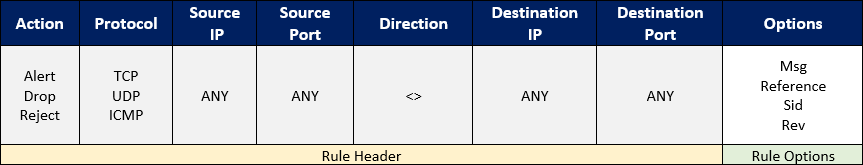
\includegraphics[width=14cm]{figure/snort_rules.png}
        \end{tabular}
    \end{center}
    \caption{Regola di Snort}
\end{figure}

L'header comprende a sua volta diversi campi:

\begin{itemize}
    \item \textbf{Action} alert, drop (blocca e logga), reject (blocca logga e termina la connessione)
    \item \textbf{Protocol} tcp,udp,icmp
    \item \textbf{Source IP}  any, un intervallo di ip, uno specifico ip
    \item \textbf{Source port} any, un range di porte,una porta
    \item \textbf{Direction} -> se si è interessati esclusivamente ai pacchetti che partono dal source ip e arrivano al destination ip, <> se si è interessati ai traffico in ambi i sensi.
    \item \textbf{Destination IP} any, un intervallo di ip, uno specifico ip.
    \item \textbf{Destination port} any, un range di porte,una porta.
\end{itemize}

L'options invece:

\begin{itemize}
    \item \textbf{msg}  è il messaggio che compare a schermo o nei log.
    \item \textbf{reference} riferimento a un CVE (Common Vulnerabilities and Exposures).
    \item \textbf{sid} l'id della rule. Deve essere un numero > di 1000000, le regole al di sotto sono riservate.
    \item \textbf{rev} informazioni sulla modifica o l'update della regola. Se rev:1 la regola non è mai stata revisionata.
\end{itemize}

Esempio:

\begin{verbatim}
alert icmp ant any -> 10.222.111.2 any (msg:"ICMP test detected"; 
sid:1000001; rev:001;)
\end{verbatim}

Snort manda un alert per i pacchetti che hanno source-ip: any, source-port: any, destination-ip: 10.222.111.2, destination-port: any.

Infine il campo options delle regole può contenere un payload, oppure dei flags per distinguere i FIN, SYN, ACK

Ad esempio:

\begin{verbatim}
alert tcp any any <> any 80 (msg: "GET Request Found"; content:"GET";
sid: 100001; rev:1;)
\end{verbatim}

Crea un alert per le GET http.

\begin{verbatim}
alert tcp any any <> any any (msg: "FLAG TEST"; flags:S; sid: 100001; rev:1;)
\end{verbatim}

Crea un alert per i SYN.

\section{Alert e log}

Comprendere il meccanismo di alerting e logging di Snort può facilitare l'apprendimento dell'intero funzionamento del sistema di rilevazione. A seguire sono mostrati alcuni dei principali strumenti di appoggio che permettono la corretta creazione dei file di log e registrazione dei pacchetti.

\subsection{Libpcap, Libnet, tcpdump}

Libpcap, Libnet, tcpdump sono API che permettono di costruire iniettare e gestire pacchetti di rete, svolgono il ruolo di packet analyzer. Vengono utilizzate per acquisire o inviare pacchetti da un dispositivo di rete live o da un file.

\subsection{DAQ}

Snort introduce il DAQ, Data Acquisition System. Il DAQ sostituisce le chiamate dirette alle funzioni libpcap che si occupano della cattura dei pacchetti, per conentire un livello di astrazione che faciliti il funzionamento di Snort.

\subsection{Pcap}

Pcap è la libreria DAQ predefinita. Se snort viene eseguito senza argomenti DAQ, funzionerà utilizzando questo modulo. Pcap si occupa della cattura dei pacchetti che verranno poi successivamente analizzati.

\subsection{Unified2}

Uno dei formati di file binario in cui possono essere registrati i pacchetti si chiama ``Unified2''. Unified2 è anche il nome del parser che consente di elaborare i log in oggetti python. Lo scopo principale è estrarre i dati di un pacchetto dal log ~\cite{Snort:2020} ~\cite{manual-snort} ~\cite{manual-snort}..

